\section{Atividade 2: Simulação com Xcos}
\subsection{Descrição do Modelo e Ferramentas}
Nesta atividade, utilizamos o Xcos, uma ferramenta gráfica do Scilab para a simulação de sistemas dinâmicos. O Xcos permite a construção de diagramas de blocos que facilitam a visualização e implementação do sistema massa-mola-amortecedor com diferentes entradas e condições iniciais.

\subsection{Parâmetros do Sistema}
O sistema é descrito pelos seguintes parâmetros, que são consistentes com os usados na Atividade 1:
\begin{itemize}
    \item Massa (\( m \)): 10 kg
    \item Coeficiente de amortecimento (\( C \)): 7 Ns/m
    \item Constante da mola (\( K \)): 5 N/m
\end{itemize}

\subsection{Condições Iniciais de Simulação}
As simulações foram executadas sob várias condições iniciais para explorar a resposta do sistema sob diferentes estados iniciais. A seguir estão as condições iniciais utilizadas, incluindo uma condição inicial adicional específica para esta atividade (Caso 0):

\begin{center}
    \begin{tabular}{|c|c|c|}
        \hline
        \textbf{Caso} & \textbf{Velocidade Inicial \( V_0 \)} & \textbf{Posição Inicial \( X_0 \)} \\
        \hline
        0             & \( 0 \, \text{m/s} \)                 & \( 0 \, \text{m} \)                \\
        1             & \( 5 \, \text{m/s} \)                 & \( 0 \, \text{m} \)                \\
        2             & \( 0 \, \text{m/s} \)                 & \( 2.5 \, \text{m} \)              \\
        3             & \( 3.33 \, \text{m/s} \)              & \( 2 \, \text{m} \)                \\
        \hline
    \end{tabular}
\end{center}

Esta tabela facilita a referência rápida às condições iniciais para cada caso simulado, permitindo uma comparação mais direta entre os diferentes cenários testados.

\subsection{Diagrama de Blocos no Xcos}
\begin{figure}[H]
    \centering
    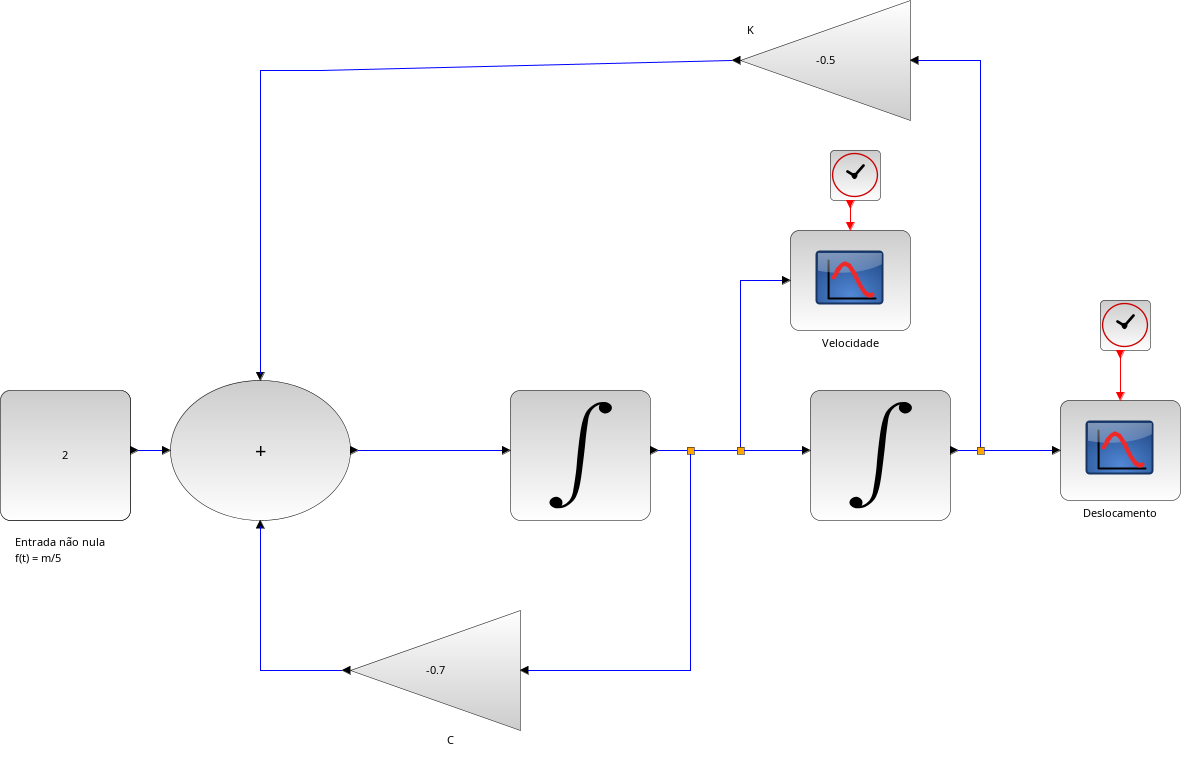
\includegraphics[width=0.8\textwidth]{final/2-atividade/assets/diagrama.png}
    \caption{Diagrama de blocos utilizado na simulação no Xcos.}
\end{figure}

\subsection{Resultados e Análise}


% Caso 0 =========================================================
\subsubsection{Análise dos Resultados para o Caso 0}
No Caso 0, analisamos a resposta do sistema quando ele parte de condições completamente estáticas (\(V_0 = 0 \, \text{m/s}\) e \(X_0 = 0 \, \text{m}\)). Esta configuração é vital para avaliar a resposta pura do sistema a uma entrada controlada sem influência inicial de deslocamento ou velocidade.

\paragraph{Deslocamento}
\begin{figure}[H]
    \centering
    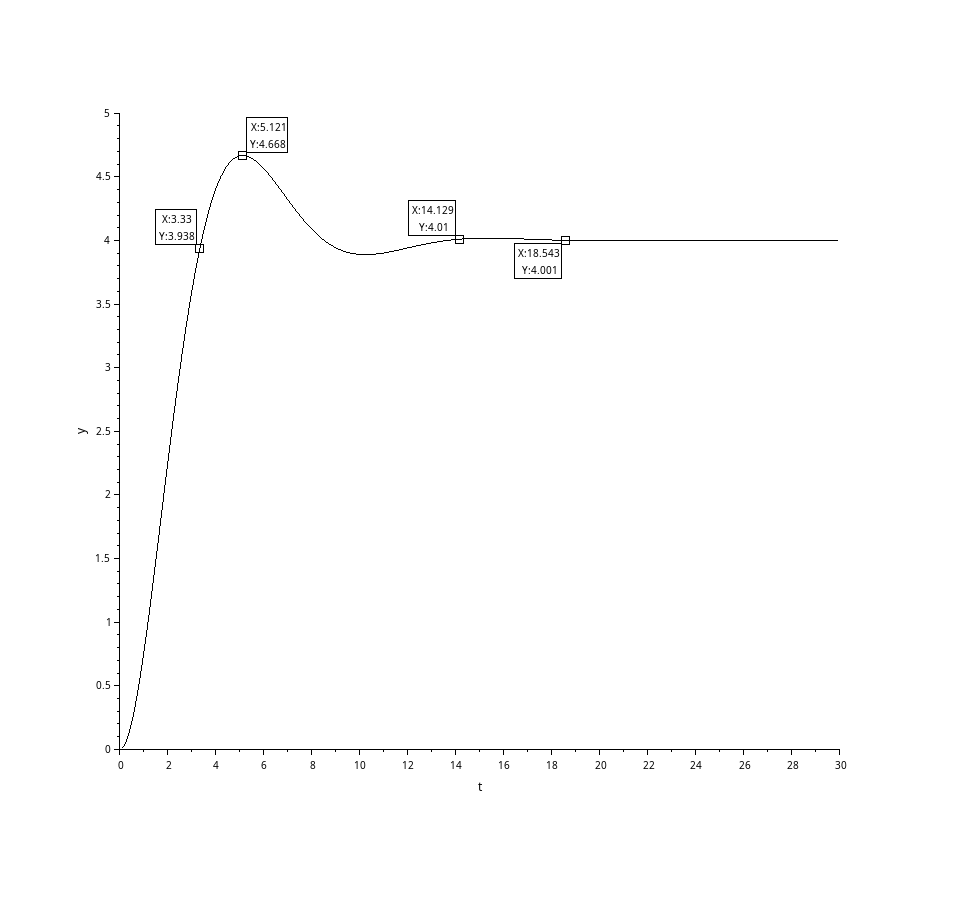
\includegraphics[height=0.7\textwidth]{final/2-atividade/assets/deslocamento-caso-0.png}
    \caption{Gráfico de deslocamento para o Caso 0.}
\end{figure}
O gráfico de deslocamento revela um pico máximo de aproximadamente 4.7 unidades aos 5.1 segundos, marcando o tempo de pico. O tempo de subida, definido como o intervalo para atingir o primeiro pico máximo a partir do repouso, é, portanto, cerca de 5.1 segundos. Após atingir o pico, o sistema exibe oscilações amortecidas que rapidamente reduzem em amplitude. O tempo de estabelecimento, onde as oscilações ficam dentro de uma faixa de ±2\% do valor final, é aproximadamente de 18 segundos, após o qual o sistema entra em uma zona estacionária, indicando estabilidade.

\paragraph{Velocidade}

\begin{figure}[H]
    \centering
    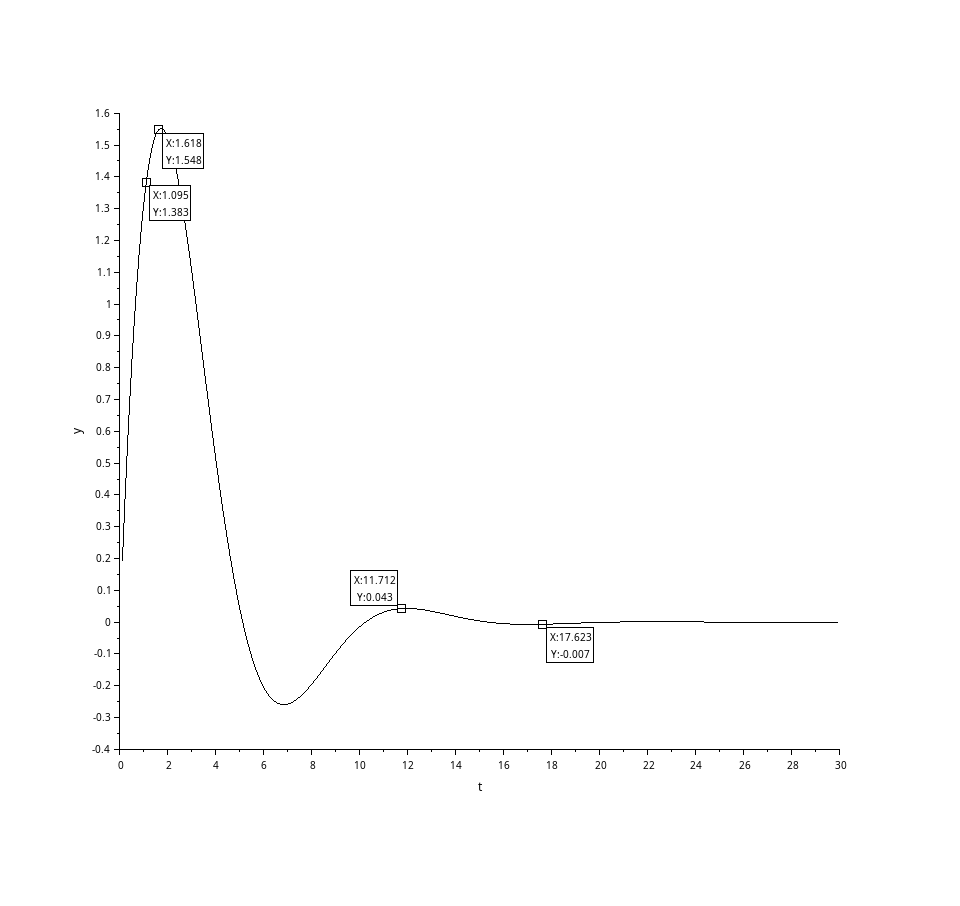
\includegraphics[height=0.7\textwidth]{final/2-atividade/assets/velocidade-caso-0.png}
    \caption{Gráfico de velocidade para o Caso 0.}
\end{figure}
O gráfico de velocidade reflete a resposta imediata do sistema à força aplicada. A velocidade atinge um pico negativo de cerca de -1.54 unidades em torno de 6.2 segundos, o que corresponde ao tempo de pico para a velocidade. A velocidade oscila abaixo e acima de zero, indicando a resposta oscilatória do sistema ao deslocamento. As oscilações diminuem progressivamente e o sistema alcança a zona estacionária por volta de 18 segundos, estabilizando-se completamente em zero.

\paragraph{Comentários Gerais}
A análise do Caso 0 mostra como o sistema responde a um estímulo externo na ausência de condições iniciais de energia. Os parâmetros transitórios, como tempo de subida, pico, e de estabelecimento, juntamente com a observação da zona estacionária, são cruciais para entender a dinâmica do sistema e a eficácia do amortecimento em trazer o sistema de volta ao repouso, minimizando oscilações excessivas. Este caso estabelece uma base comparativa para outros casos com condições iniciais variadas.


% Caso 1 =========================================================
\subsubsection{Análise dos Resultados para o Caso 1}
No Caso 1, analisamos a resposta do sistema quando ele parte com uma velocidade inicial significativa (\(V_0 = 5 \, \text{m/s}\)) e sem deslocamento inicial (\(X_0 = 0 \, \text{m}\)). Esta condição inicial permite avaliar como uma energia cinética inicial afeta a resposta dinâmica do sistema, especialmente em termos de deslocamento máximo e oscilações resultantes.


\paragraph{Deslocamento}
\begin{figure}[H]
    \centering
    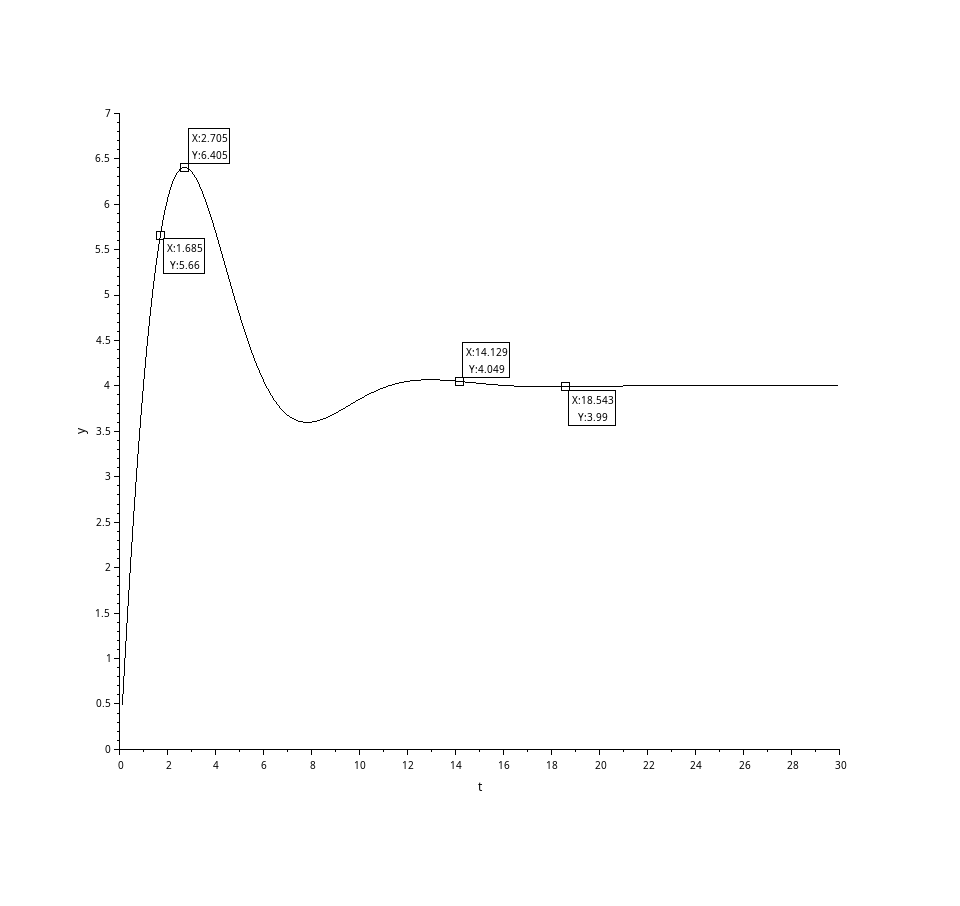
\includegraphics[height=0.7\textwidth]{final/2-atividade/assets/deslocamento-caso-1.png}
    \caption{Gráfico de deslocamento para o Caso 1.}
\end{figure}
O gráfico mostra que o sistema parte de zero e rapidamente atinge um pico de aproximadamente 6.5 unidades ao redor de 2.7 segundos, refletindo uma resposta aguda à velocidade inicial. Esse pico é seguido por uma diminuição significativa, que desce abaixo do zero antes de estabilizar. O tempo de subida é rapidamente alcançado, enquanto o tempo de estabelecimento, onde as oscilações permanecem dentro de uma faixa de ±2\% do valor estacionário final, é observado por volta de 18 segundos.


\paragraph{Velocidade}
\begin{figure}[H]
    \centering
    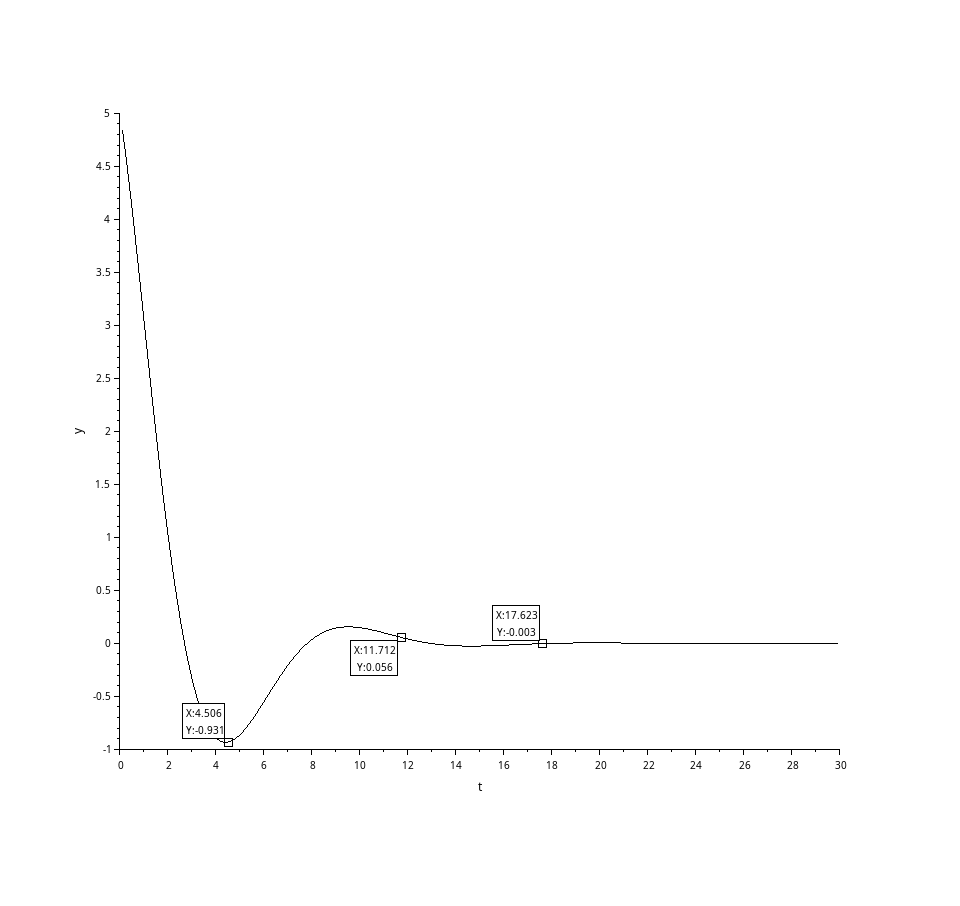
\includegraphics[height=0.7\textwidth]{final/2-atividade/assets/velocidade-caso-1.png}
    \caption{Gráfico de velocidade para o Caso 1.}
\end{figure}
A velocidade inicialmente picos a uma taxa significativa, refletindo o impulso inicial aplicado. O pico máximo de velocidade ocorre quase simultaneamente com o pico de deslocamento, marcando -1.54 unidades em torno de 1.68 segundos. Após atingir este pico, a velocidade oscila e gradualmente se aproxima de zero, indicando que o sistema está alcançando uma zona estacionária por volta de 18 segundos, semelhante ao observado no deslocamento.


\paragraph{Comentários Gerais}
A análise do Caso 1 ilustra como a condição inicial de velocidade influencia a resposta dinâmica do sistema massa-mola-amortecedor. Os parâmetros transitórios, como o tempo de subida e o tempo de pico, são drasticamente diferentes em comparação com o Caso 0, onde não havia energia cinética inicial. Isso destaca a importância de considerar condições iniciais variadas para entender completamente o comportamento do sistema em diferentes cenários de operação. Este caso também reforça o papel crítico do amortecimento na estabilização do sistema após perturbações iniciais.


% Caso 2 =========================================================
\subsubsection{Análise dos Resultados para o Caso 2}
No Caso 2, analisamos a resposta do sistema quando ele parte com um deslocamento inicial (\(X_0 = 2.5 \, \text{m}\)) e sem velocidade inicial (\(V_0 = 0 \, \text{m/s}\)). Esta configuração é fundamental para entender como o sistema responde a uma perturbação inicial na posição sem impulso inicial.

\paragraph{Deslocamento}
\begin{figure}[H]
    \centering
    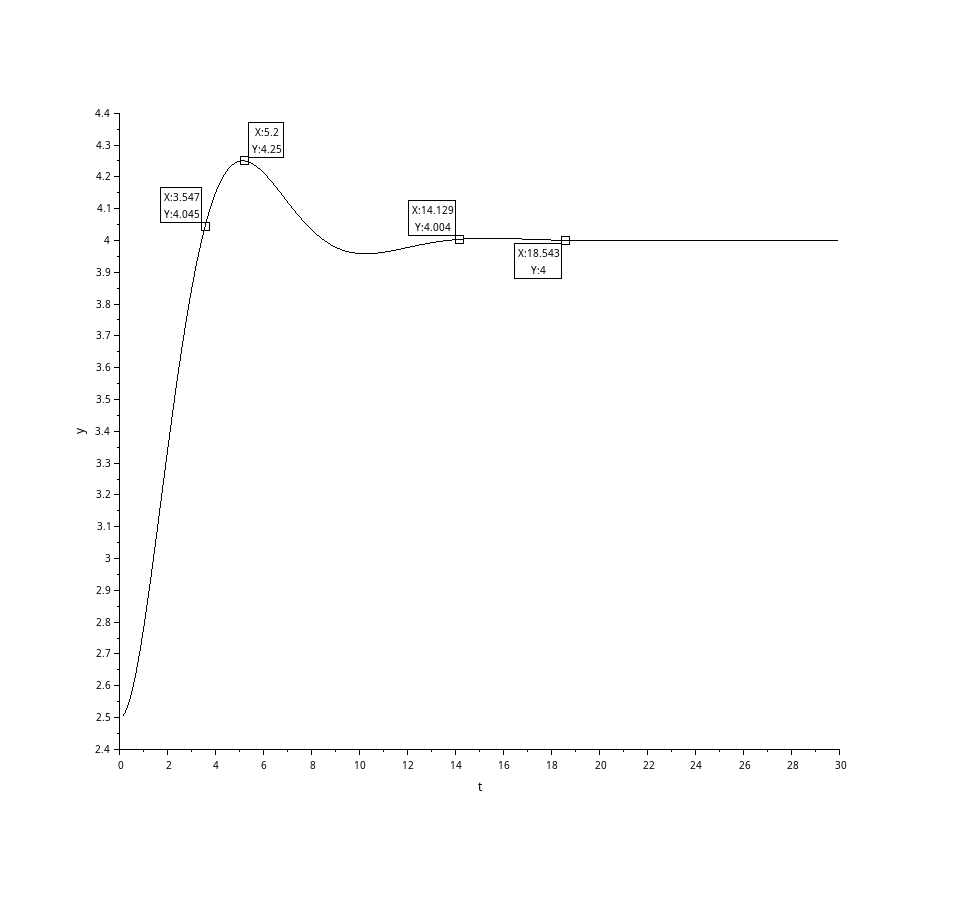
\includegraphics[height=0.7\textwidth]{final/2-atividade/assets/deslocamento-caso-2.png}
    \caption{Gráfico de deslocamento para o Caso 2.}
\end{figure}
O gráfico de deslocamento mostra que o sistema parte de um deslocamento inicial de 2.5 m, rapidamente atinge um pico de cerca de 4.25 m aos 5.2 segundos, indicando a resposta máxima do sistema ao ser liberado. Após esse pico, o sistema exibe oscilações que rapidamente se amortecem, com o deslocamento oscilando abaixo e acima do zero, estabilizando-se finalmente em torno do zero. O tempo de estabelecimento, onde as oscilações permanecem dentro de uma faixa de ±2\% do valor final, é aproximadamente de 18 segundos.

\paragraph{Velocidade}
\begin{figure}[H]
    \centering
    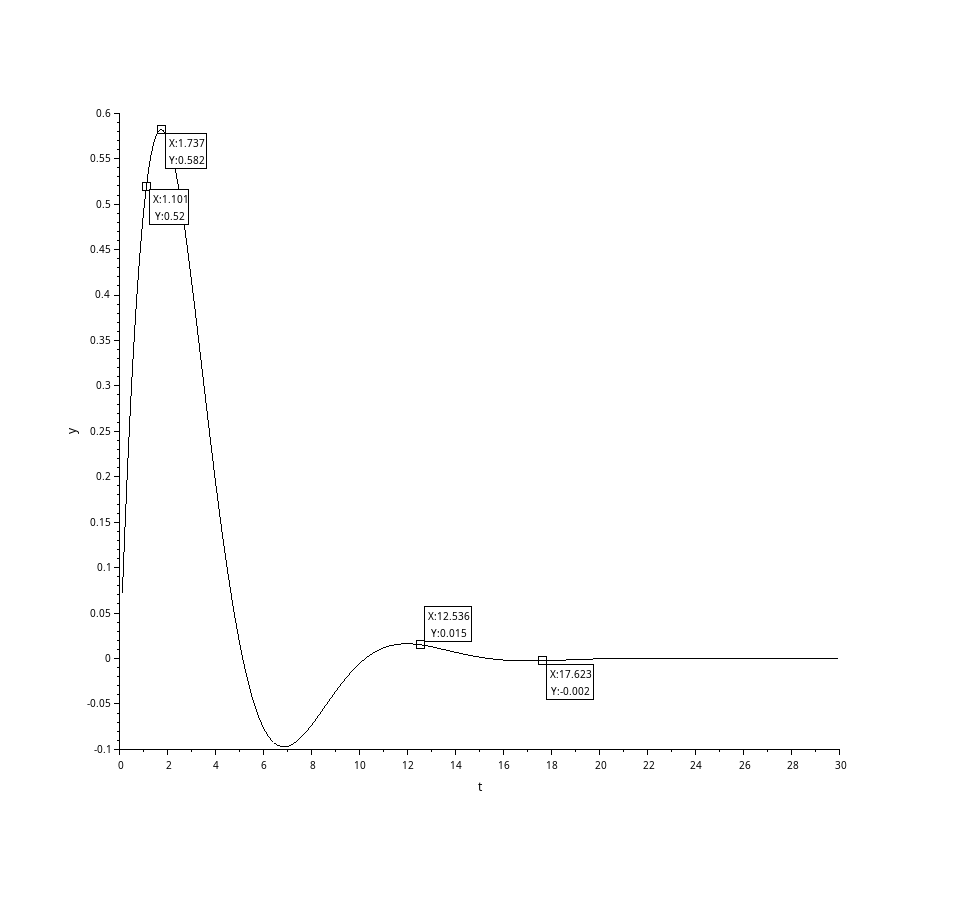
\includegraphics[height=0.7\textwidth]{final/2-atividade/assets/velocidade-caso-2.png}
    \caption{Gráfico de velocidade para o Caso 2.}
\end{figure}
A velocidade inicialmente aumenta à medida que o sistema se move de volta para a posição de equilíbrio, atingindo um pico negativo de -0.52 m/s logo após o início, correspondente à velocidade máxima ao passar pelo equilíbrio na direção oposta ao deslocamento inicial. A velocidade então oscila, diminuindo em magnitude devido ao amortecimento, até estabilizar-se em zero. O sistema atinge uma zona estacionária com velocidade quase nula, demonstrando a eficácia do amortecimento em dissipar a energia cinética inicialmente induzida pelo deslocamento.

\paragraph{Comentários Gerais}
O Caso 2 destaca a resposta do sistema a um teste de posição, com deslocamento inicial sem velocidade inicial. Os resultados mostram claramente como a energia potencial armazenada é convertida em energia cinética, e como o amortecimento é crucial para a estabilização do sistema. Este caso também é importante para verificar a eficácia do sistema em retornar ao repouso sem oscilações residuais prolongadas, essencial em aplicações práticas onde respostas rápidas e estabilizadas são necessárias.

% Caso 3 =========================================================
\subsubsection{Análise dos Resultados para o Caso 3}
No Caso 3, analisamos a resposta do sistema quando ele parte com uma velocidade inicial (\(V_0 = 3.33 \, \text{m/s}\)) e um deslocamento inicial (\(X_0 = 2 \, \text{m}\)). Esta combinação de condições iniciais é significativa para explorar a resposta dinâmica sob energia cinética e potencial simultâneas.

\paragraph{Deslocamento}
\begin{figure}[H]
    \centering
    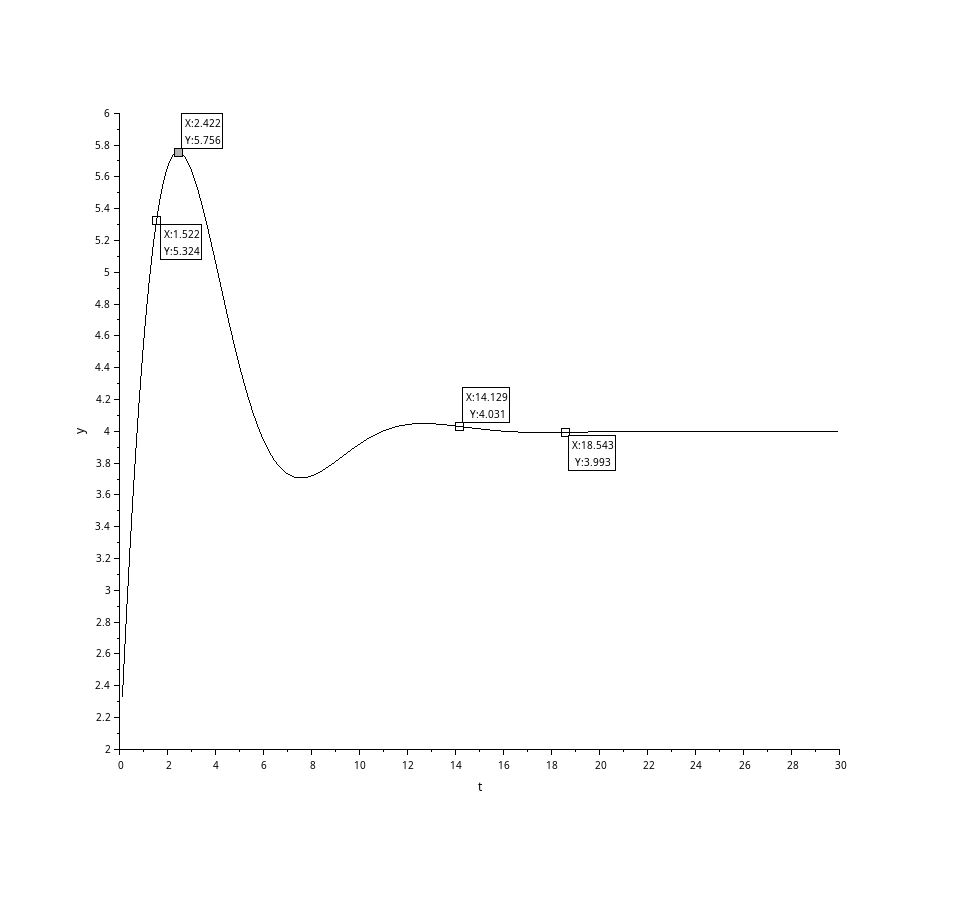
\includegraphics[height=0.7\textwidth]{final/2-atividade/assets/deslocamento-caso-3.png}
    \caption{Gráfico de deslocamento para o Caso 3.}
\end{figure}
O gráfico de deslocamento mostra que o sistema começa com um impulso inicial que o leva a um pico de aproximadamente 5.75 m ao redor de 2.4 segundos. Após esse pico, o sistema exibe oscilações que reduzem gradualmente em amplitude devido ao amortecimento. O sistema estabiliza perto do zero, com o tempo de estabelecimento aproximadamente em 18 segundos, onde as oscilações ficam dentro de uma faixa aceitável indicando uma zona estacionária.

\paragraph{Velocidade}
\begin{figure}[H]
    \centering
    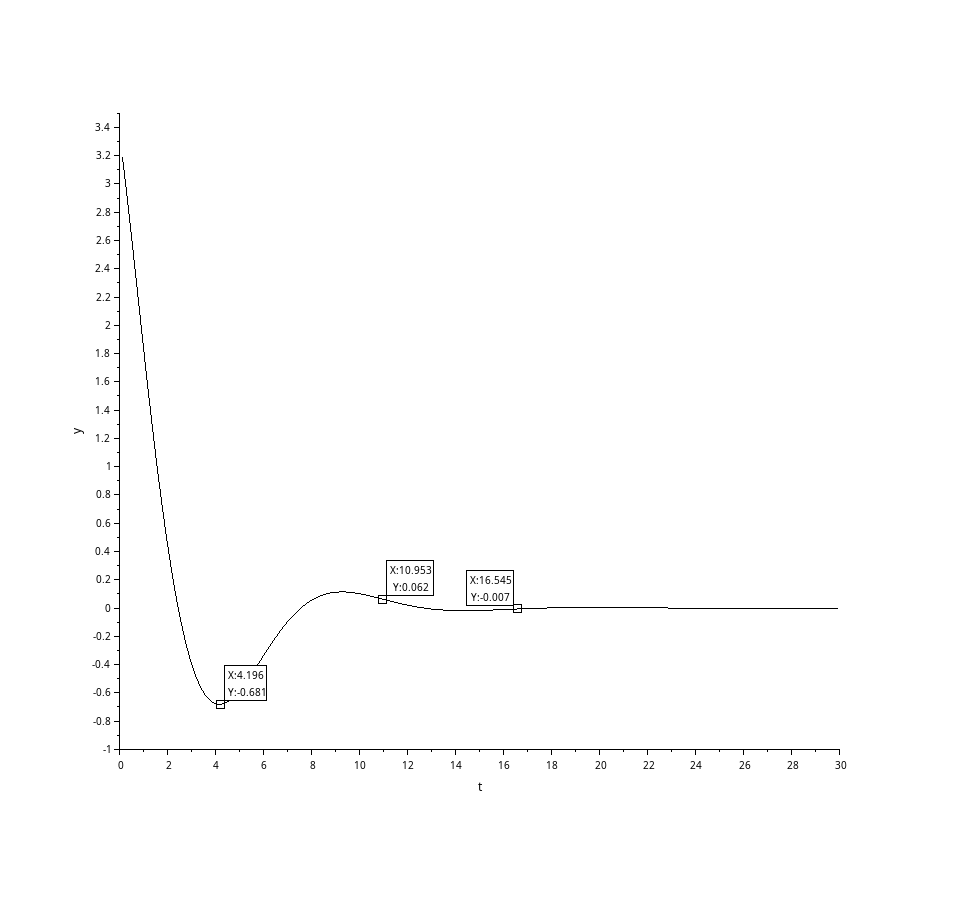
\includegraphics[height=0.7\textwidth]{final/2-atividade/assets/velocidade-caso-3.png}
    \caption{Gráfico de velocidade para o Caso 3.}
\end{figure}
A velocidade inicialmente mostra uma rápida ascensão, atingindo um pico de aproximadamente 5.32 m/s. Essa alta velocidade inicial contribui para o rápido pico de deslocamento observado. A velocidade então oscila, diminuindo progressivamente até estabilizar-se em torno de zero. A estabilização final da velocidade é alcançada em torno de 18 segundos, refletindo a eficácia do amortecimento e a interação entre as forças restauradoras e o amortecimento.

\paragraph{Comentários Gerais}
O Caso 3 oferece uma perspectiva complexa sobre a dinâmica do sistema quando energias cinética e potencial são ambas significativas desde o início. As oscilações observadas e a subsequente estabilização demonstram como diferentes tipos de energia inicial influenciam a resposta do sistema e a eficácia do amortecimento em controlar a resposta até a estabilidade. Este caso é particularmente útil para entender a resposta do sistema em condições iniciais variadas e complexas, sendo essencial para aplicações práticas onde o sistema pode ser sujeito a perturbações iniciais múltiplas.

% Conclusão
\subsection{Conclusão Geral dos Casos Estudados}

Ao longo desta atividade, analisamos as respostas do sistema massa-mola-amortecedor sob várias condições iniciais, abrangendo os Casos 0 a 3. Cada caso foi projetado para ilustrar aspectos diferentes da dinâmica do sistema, considerando diferentes combinações de deslocamento e velocidade iniciais.

\paragraph{Observações Gerais}

Os casos estudados mostraram uma ampla gama de comportamentos dinâmicos:
\begin{itemize}
    \item \textbf{Caso 0} serviu como um ponto de referência, onde o sistema partiu do repouso sem energia inicial, permitindo observar a resposta pura à força aplicada.
    \item \textbf{Caso 1} demonstrou a influência de uma velocidade inicial significativa, ilustrando como a energia cinética influencia as oscilações e a estabilidade subsequente do sistema.
    \item \textbf{Caso 2} focou no efeito de um deslocamento inicial sem velocidade, enfatizando a conversão de energia potencial em energia cinética e vice-versa.
    \item \textbf{Caso 3} combinou tanto deslocamento quanto velocidade iniciais, mostrando a interação complexa entre as duas formas de energia desde o início da simulação.
\end{itemize}

Durante as simulações, os parâmetros do sistema foram mantidos constantes para garantir a consistência dos resultados, permitindo uma comparação direta entre os diferentes casos. Os resultados foram meticulosamente analisados para observar o comportamento transiente e a estabilidade a longo prazo, utilizando métricas como tempo de subida, tempo de pico e tempo de estabelecimento. As oscilações foram avaliadas para determinar a eficácia do amortecimento em dissipar a energia e estabilizar o sistema.

\paragraph{Conclusões da Análise}
Esta atividade sublinhou a importância de compreender a dinâmica de sistemas massa-mola-amortecedor em várias configurações iniciais. As simulações forneceram insights valiosos sobre como diferentes condições iniciais afetam a resposta do sistema e como o design adequado do amortecimento e da rigidez da mola é crucial para o comportamento desejado. A abordagem utilizada garantiu que todas as premissas da atividade fossem cumpridas, fornecendo uma base sólida para futuras investigações e aplicações práticas dos princípios estudados.
